\chapter{Unmanned Aerial Vehicles}\label{ch:unmanned_aerial_vehicles}

The term \gls{uav} encompasses a diverse range of aircraft, from compact quad-copters to larger fixed-wing models. What primarily distinguishes \glspl{uav} from conventional aircraft is that \glspl{uav} are either remotely piloted or autonomously controlled, whereas traditional aircraft are operated by human pilots. This autonomy enables \glspl{uav} to be deployed in scenarios where human presence is either impractical or hazardous, such as military operations or environments with significant risk.

\glspl{uav} serve various purposes across multiple industries, including surveillance, reconnaissance, search and rescue missions, and scientific research. Additionally, they have become invaluable in sectors like agriculture, forestry, and environmental monitoring. In recent years, \glspl{uav} have gained popularity among hobbyists for recreational flying and personal projects.

\section{Types of Unmanned Aerial Vehicles}\label{sec:uav_types}

In line with the classification presented by the \gls{easa} \autocite{eu-947-2019}, \glspl{uav} can be categorized into three main types, each based on size, weight, physical design, and operational capabilities:

\begin{itemize}
  \item \textbf{Fixed-wing \glspl{uav}:} These aircraft feature fixed wings and function similarly to conventional airplanes. They tend to be larger and designed for long-duration flights, making them suitable for extended missions like surveillance, reconnaissance, and mapping. However, they require runways for takeoff and landing, and cannot hover in place, limiting their versatility in confined spaces.

  \item \textbf{Rotary-wing \glspl{uav}:} Equipped with multiple rotors, these \glspl{uav} can take off and land vertically. They are typically smaller and more agile, making them ideal for close-range missions like aerial photography, search and rescue, and surveillance. However, their limited range and endurance compared to fixed-wing \glspl{uav} restrict their use in long-duration missions.

  \item \textbf{Hybrid \glspl{uav}:} Combining the features of both fixed-wing and rotary-wing designs, hybrid \glspl{uav} can take off and land vertically like rotary-wing models while achieving greater range and endurance through fixed-wing flight. These aircraft are ideal for missions requiring versatility, such as reconnaissance and mapping. Despite their advantages, they are more complex and costly to operate than single-type \glspl{uav}.
\end{itemize}

\Cref{fig:uav_types} illustrates the different \glspl{uav} types based on their design and intended applications.

\begin{figure}
  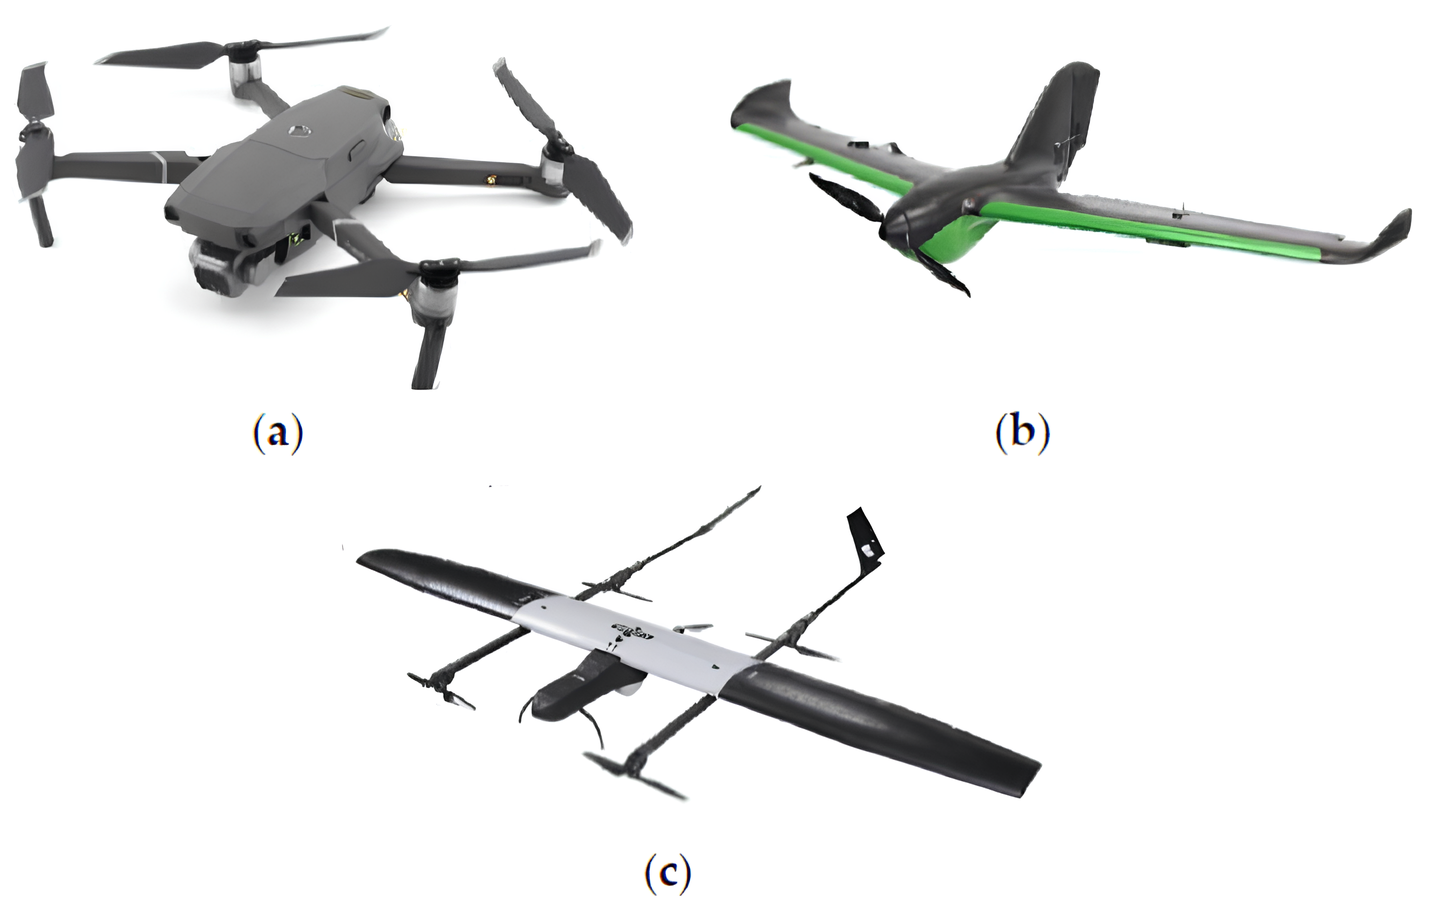
\includegraphics{uav_types.png}
  \caption{Types of \glsentryshortpl{uav} based on their design and intended use \autocite{mohnani2022role}.\ a. Rotary-wing \glsentryshort{uav}, b. Fixed-wing \glsentryshort{uav}, c. Hybrid \glsentryshort{uav}}\label{fig:uav_types}
\end{figure}

In \cref{tab:uav_categories}, a detailed comparison of fixed-wing, rotary-wing, and hybrid \glspl{uav} is presented across various performance metrics, including size, range, endurance, cost, and ease of operation. The table provides insights to help in selecting the appropriate \gls{uav} for specific mission requirements, depending on factors like payload, range, and maneuverability.

\begin{table}
  \begin{tabular}{ l c c c }
    \toprule
    \textbf{Metric} & \textbf{Fixed-wing} & \textbf{Rotary-wing} & \textbf{Hybrid} \\
    \midrule
    Size & Moderate & Small & Large \\
    Range & Long & Short & Moderate \\
    Endurance & High & Low & Moderate \\
    Payload capacity & High & Low & Moderate \\
    Maneuverability & Low & High & Moderate \\
    Ease of use & Moderate & High & Low \\
    Maintenance & Moderate & Low & High \\
    Runway requirement & Yes & No & Yes \\
    Cost & Moderate & Low & High \\
    \bottomrule
  \end{tabular}
  \caption{Comparison of fixed-wing, rotary-wing, and hybrid \glsentryshortpl{uav} across various performance metrics}\label{tab:uav_categories}
\end{table}

\section{Applications of Unmanned Aerial Vehicles}

\glspl{uav} have a wide range of applications across different industries, leveraging their versatility, maneuverability, and autonomy. Some common applications of \glspl{uav} include:

\begin{itemize}
  \item \textbf{Aerial photography and videography:} \glspl{uav} equipped with high-resolution cameras are used for capturing aerial images and videos for various purposes, including filmmaking, real estate, and landscape photography.

  \item \textbf{Agriculture:} \glspl{uav} are employed in precision agriculture to monitor crop health, assess soil conditions, and optimize irrigation and fertilization practices. They can provide valuable insights to farmers for improving crop yield and reducing resource wastage.

  \item \textbf{Search and rescue:} \glspl{uav} equipped with thermal imaging cameras and other sensors are used in search and rescue operations to locate missing persons, assess disaster-affected areas, and deliver essential supplies to remote locations.

  \item \textbf{Infrastructure inspection:} \glspl{uav} are utilized for inspecting critical infrastructure like bridges, power lines, and pipelines. They can access hard-to-reach areas and capture detailed images for assessing structural integrity and identifying maintenance needs.

  \item \textbf{Environmental monitoring:} \glspl{uav} are deployed for monitoring environmental parameters like air quality, water quality, and wildlife populations. They can collect data in remote or hazardous environments, providing valuable insights for conservation efforts and scientific research.

  \item \textbf{Disaster response:} \glspl{uav} play a crucial role in disaster response by providing real-time situational awareness, mapping affected areas, and coordinating emergency operations. They can assist in assessing damage, locating survivors, and delivering aid to disaster-stricken regions.

  \item \textbf{Military and defense:} \glspl{uav} are extensively used in military and defense applications for reconnaissance, surveillance, target acquisition, and combat operations. They offer a cost-effective and low-risk alternative to manned aircraft in high-risk environments.

    \item \textbf{Delivery services:} \glspl{uav} are increasingly being used for last-mile delivery of goods and services. Companies like Amazon and UPS are exploring the use of \glspl{uav} for delivering packages to customers in urban and rural areas.
\end{itemize}
